\chapter{Design}

In this chapter, the process of deciding upon and making the design of the Physical interface (music educational tool), will be explained. The design will be based on the formulated design requirements (see \autopageref{sec:DRequirements}), as well as common design principles (Gestalt), the SOTA (see \autopageref{sec:sota}) and knowledge gained from the workshop at Sankt Annæ (see \autopageref{sec:workshop}). 


\section{Intial design}
The design of the physical interface was, with the design requirements, not specified to the extend that a specific concept for the design was obvious. The design could instead be taken in broad variety of directions, and still live up to the requirements. As so, the design of the physical interface has been though lots of different concepts and iterations. 

\subsection {Workshop prototypes - The pre-initial designs}
In the stage of the analysis (before the Final problem statement was settled upon) where the problem concerning a lack of educational tools - build upon collaboration - was discovered, multiple initial designs was created as low fidelity prototypes. These were the ones presented at the workshop at Sankt Annæ (\autopageref{sec:workshop}). As stated (\autopageref{sec:ProblemArea}),was the protoypes in this stage, used to discuss and discover elements and concepts for which could be used in the final design. The finds from this workshop did not necessarily led to requirements, but instead served as pointers to which direction the design could be taken, when trying to achieve a tool the target group could desire. For example could the tool use movement, but it might conflict with or change focus from the learning aspect, and (in such case) should be avoided. In another case, the element (in this case movement) might serve to enhance the learning outcome (see \autopageref{AnalysisMovement}), and should therefore be strived for. This however depend on the individual concept, and each find from the workshop should therefore be discussed for each design idea. 
\\\\
In order to evaluate upon many different elements and ways of collaborating and learning music, the aim of the  concepts behind the prototypes, was differ significantly from one another. Both the topic of the material to be learned, and the way to work with this, was therefore different for each of the concepts. Each concept will be briefly described in the following, and can be found described in more detail in the appendix \todo{ref}. 
\todo{lav "collage" med ideer og giv kort beskrivelse af concept ( ryste klods,joystic band,chord master felx ,frugt løkker,quizz game )}


\subsection{From workshop and requirements - the Crawford slip method}
To evaluate upon the workshop prototype concepts in relation to the design requirements formulated and the knowledge gained from the workshop, a custom version of the Crawford slip method was used (see \autopageref{designMethod}). By doing this, a list of suggestions to how elements could be used, and should not be used, was made, and used as inspiration for other concept ideas. A sample of the list can be seen in figure \todo{lav fig og ref til den }. The full list can be seen in the appendix \autopageref{CrawfordSlipList}.  

-----------------\\\\







Alex



The group split up into two groups of 3 people. Using these pointers to make a final idea. 
The two ideas from each group can be seen in appendix …..XXXX. 
The two ideas were then discussed and talked through to finalize the final design. 

\section{Final design}
Below is the design concept sketches of the final design. 

\begin{figure}[H]
	\centering
	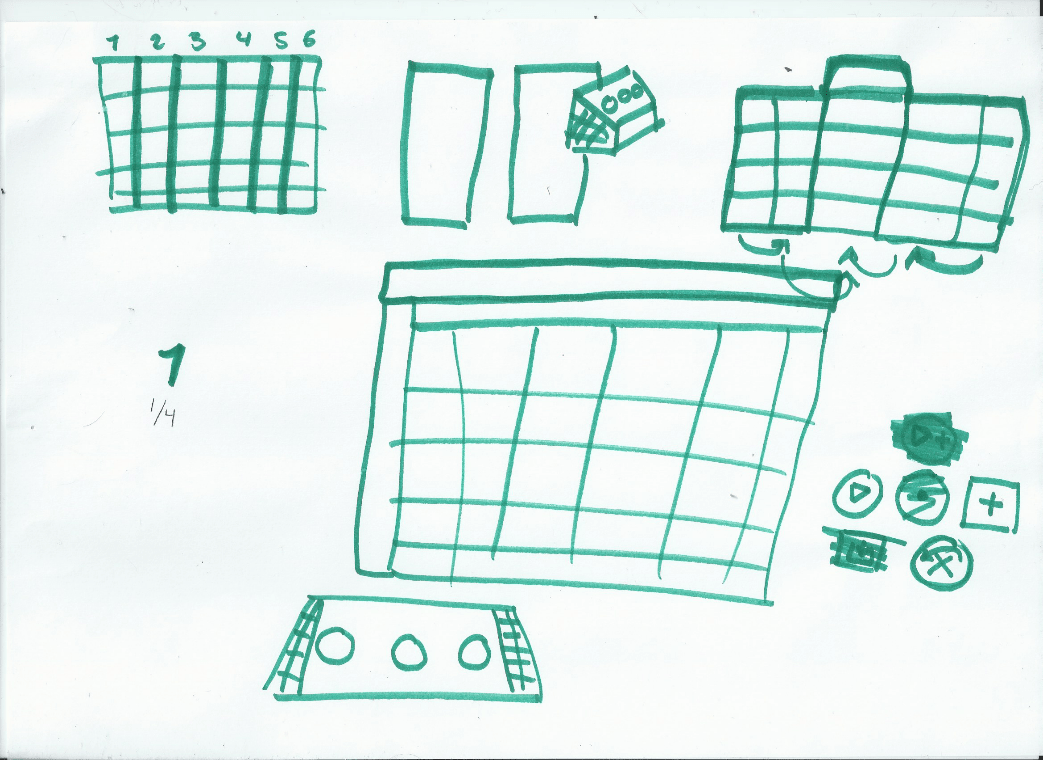
\includegraphics[width=0.7\linewidth]{figure/Design/sketchOne}
	\label{fig:sketchOne}
	\caption{Shows the early stage of the final design}
	
\end{figure}

\begin{figure}[H]
	\centering
	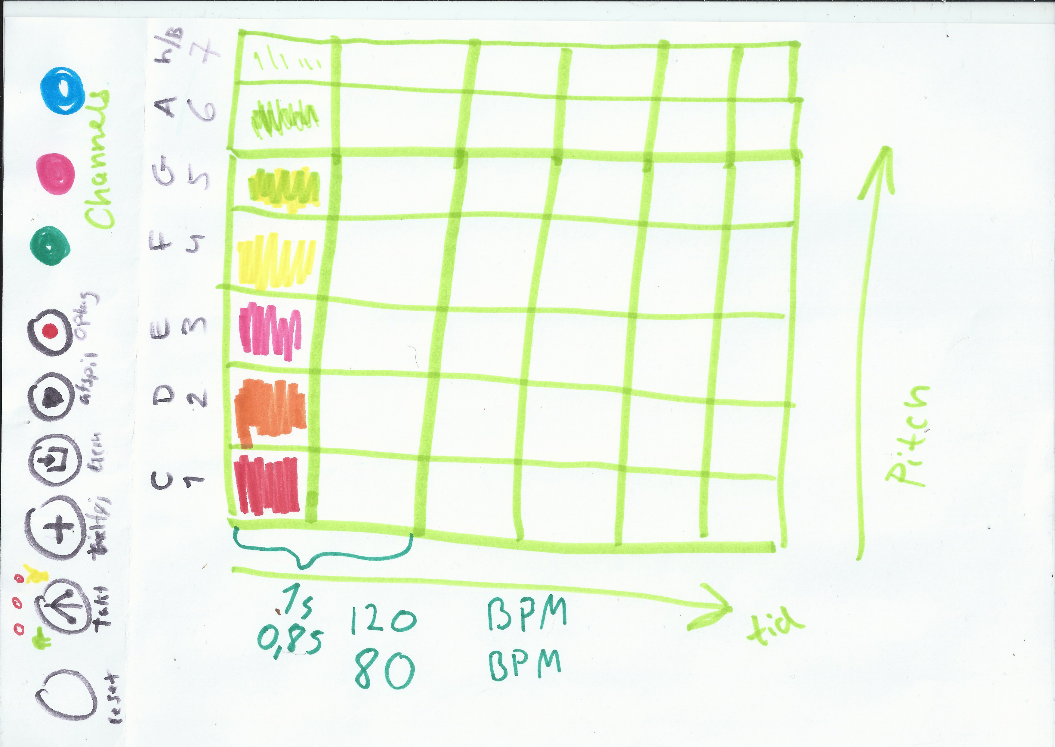
\includegraphics[width=0.7\linewidth]{figure/Design/sketchTwo}
	\label{fig:sketchTwo}
	\caption{Shows the the more completed final design}
	
\end{figure}

\begin{figure}[H]
	\centering
	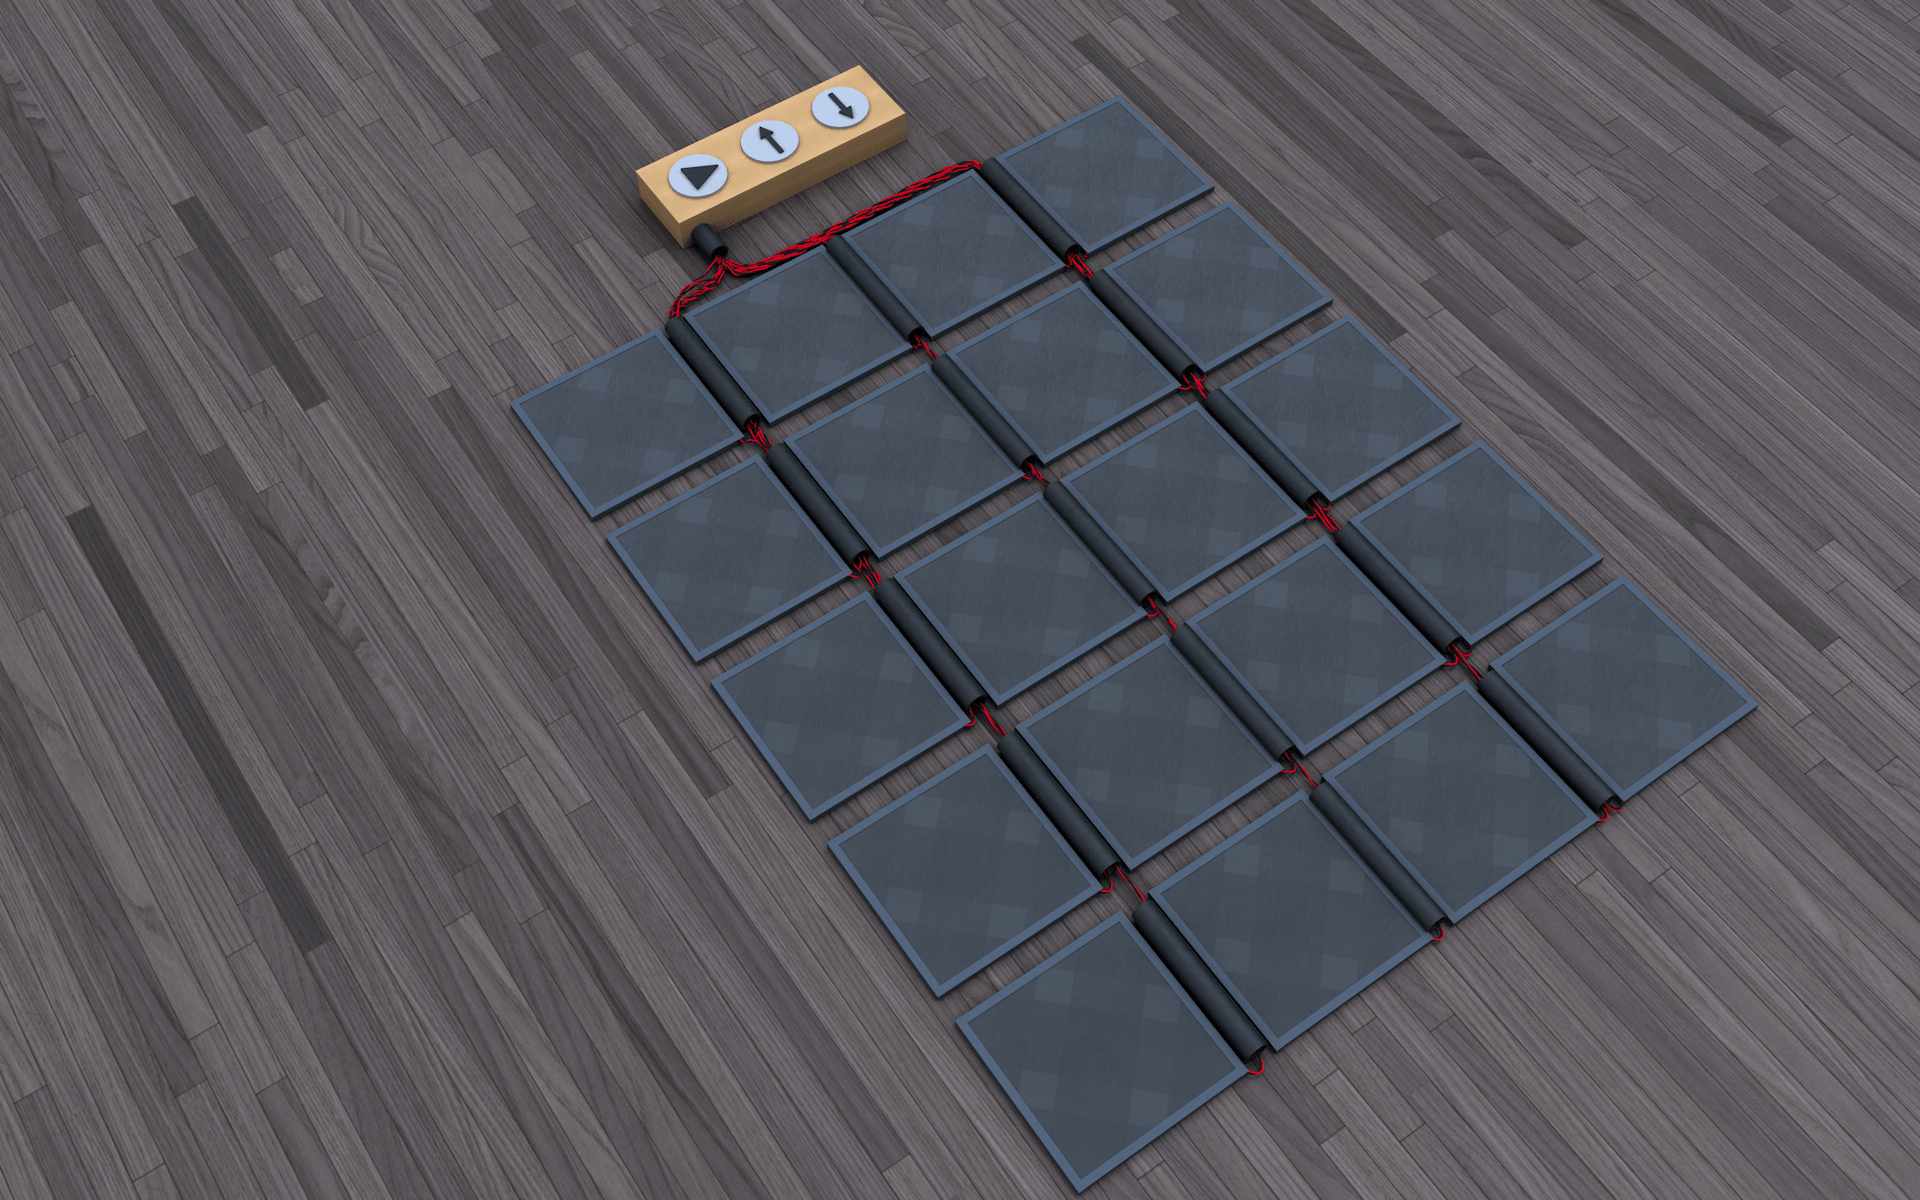
\includegraphics[width=0.7\linewidth]{figure/Design/finaldesign}
	\label{fig:finaldesign}
	\caption{The picture of how the final design should look like}
	
\end{figure}


\section{The physical interface}

\subsection{Making of the buttons}

The process of the buttons used for the interaction with the mat.

\begin{figure}[H]
	\centering
	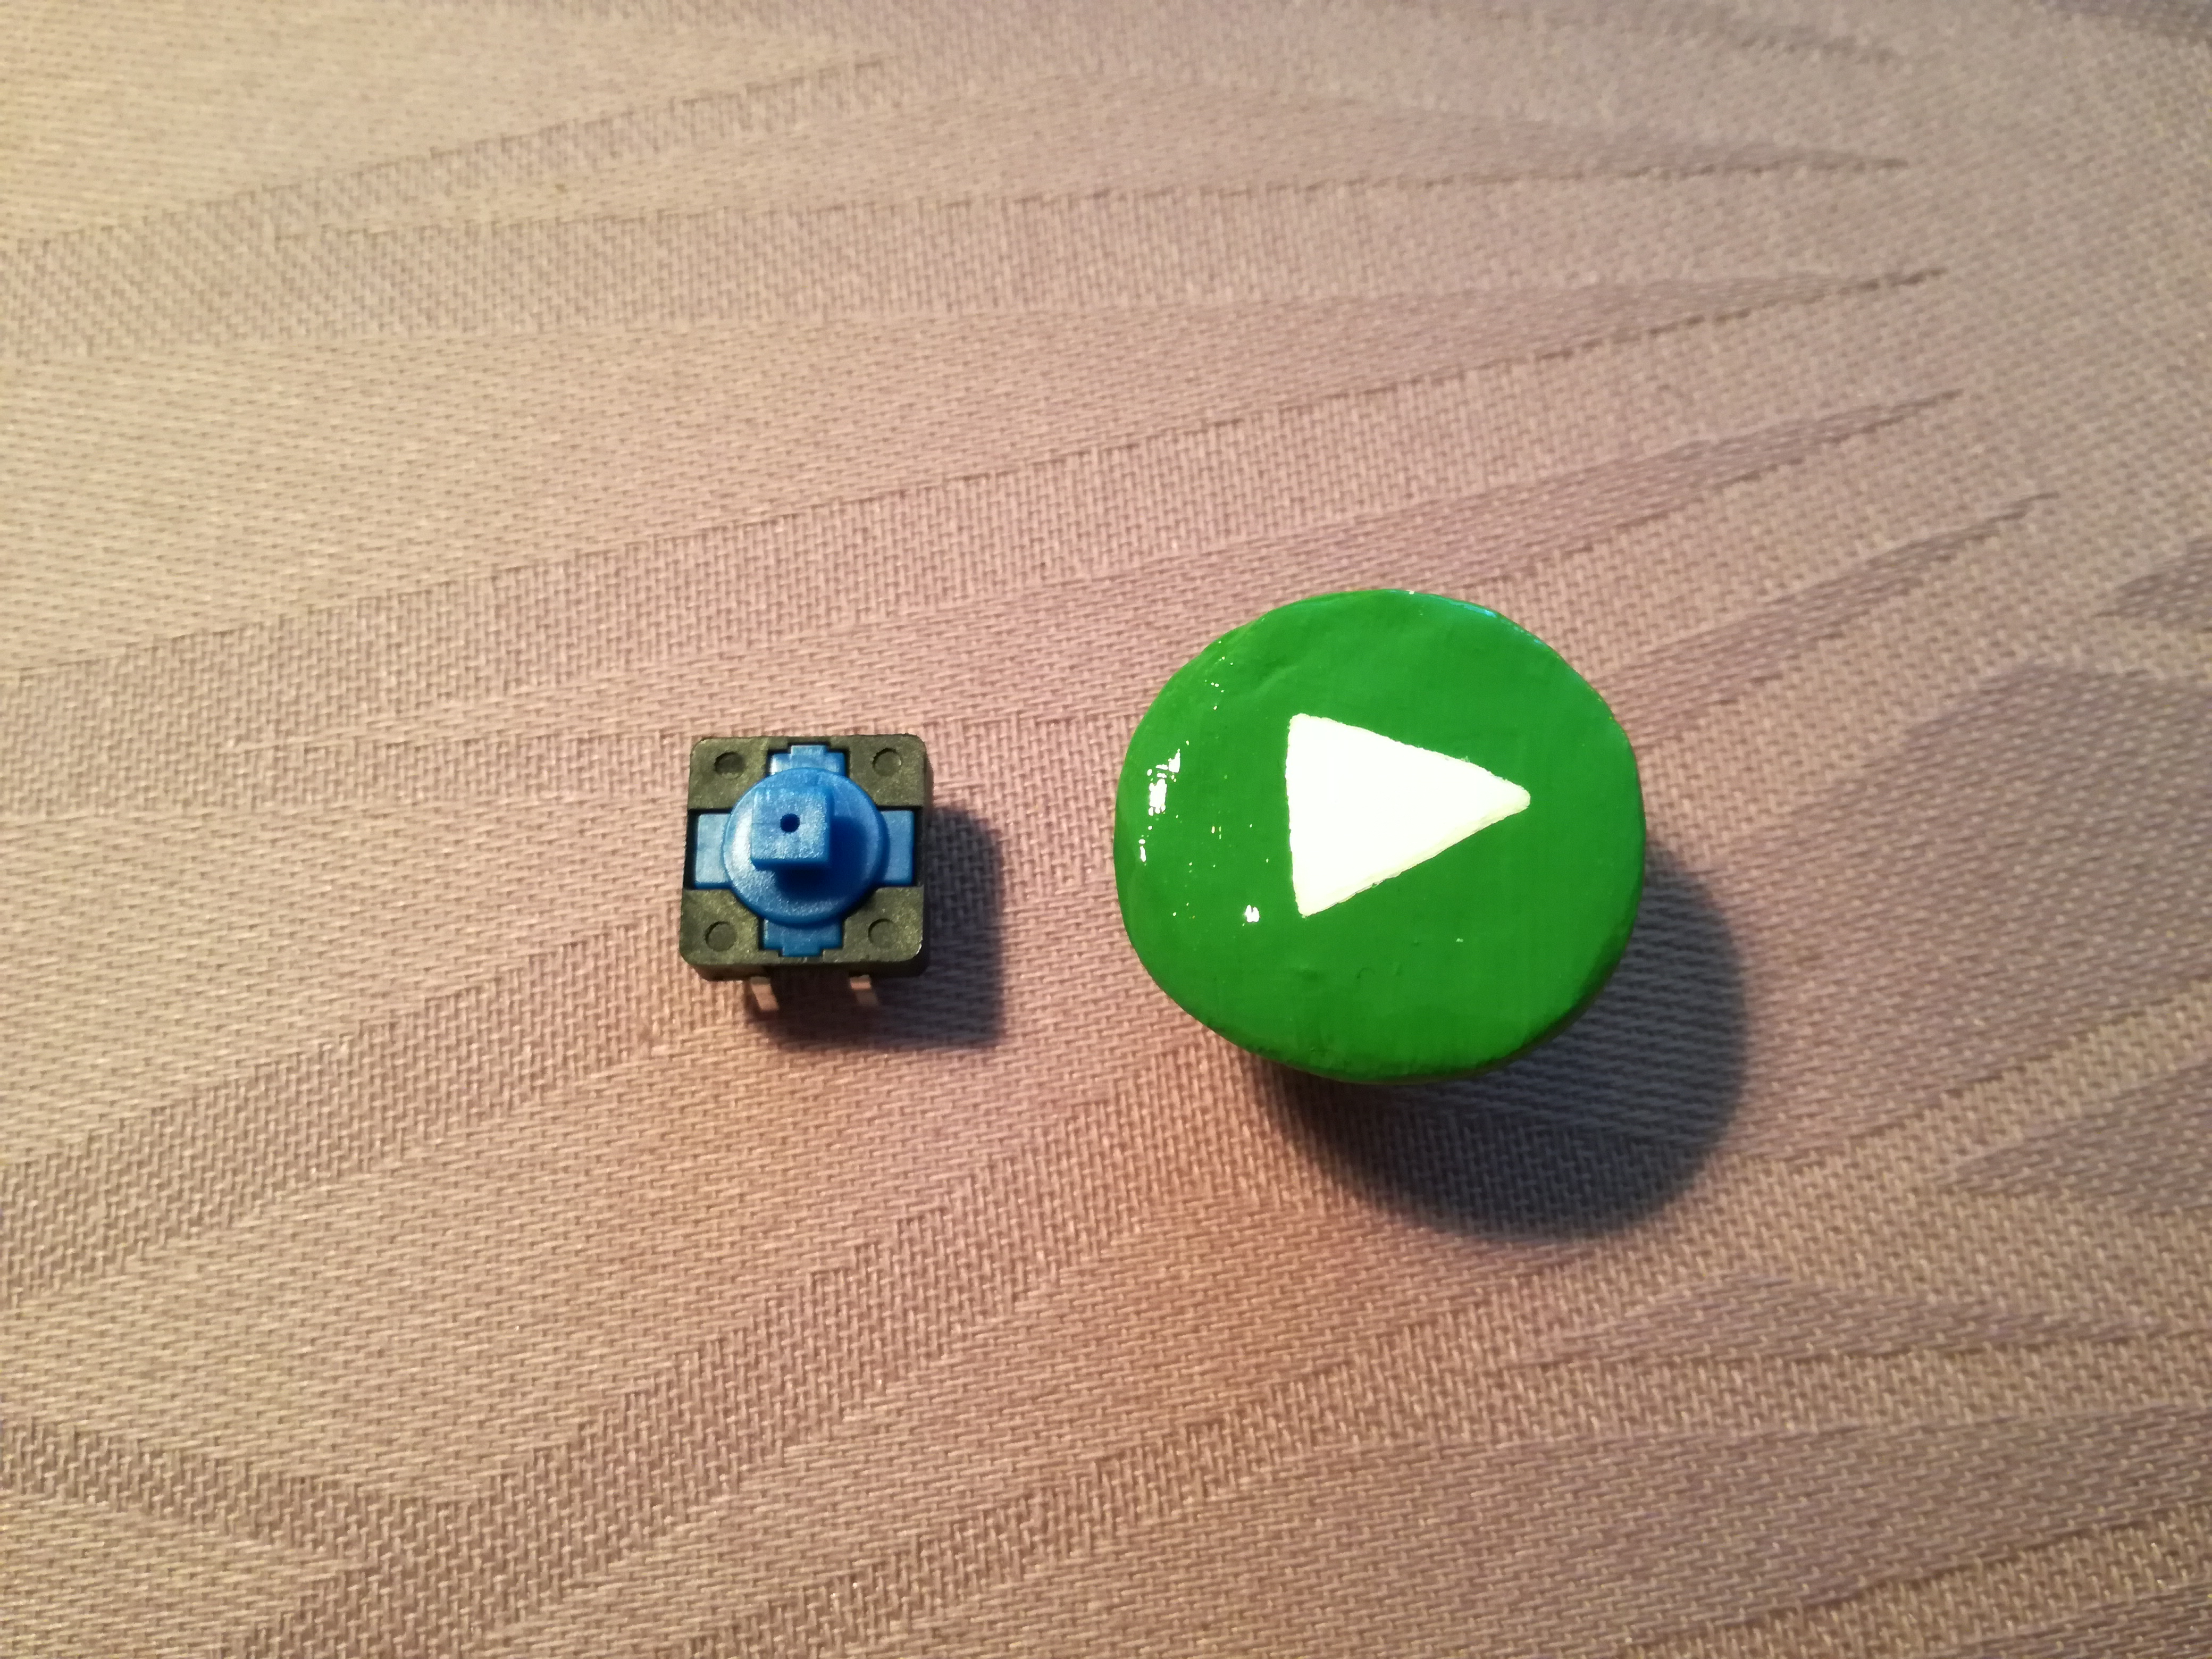
\includegraphics[width=0.7\linewidth]{figure/Design/buttons}
	\label{fig:buttons}
	\caption{On the left is the button without the customized button and on the right is the customized version of the final play button.}
	
\end{figure}

\begin{figure}[H]
	\centering
	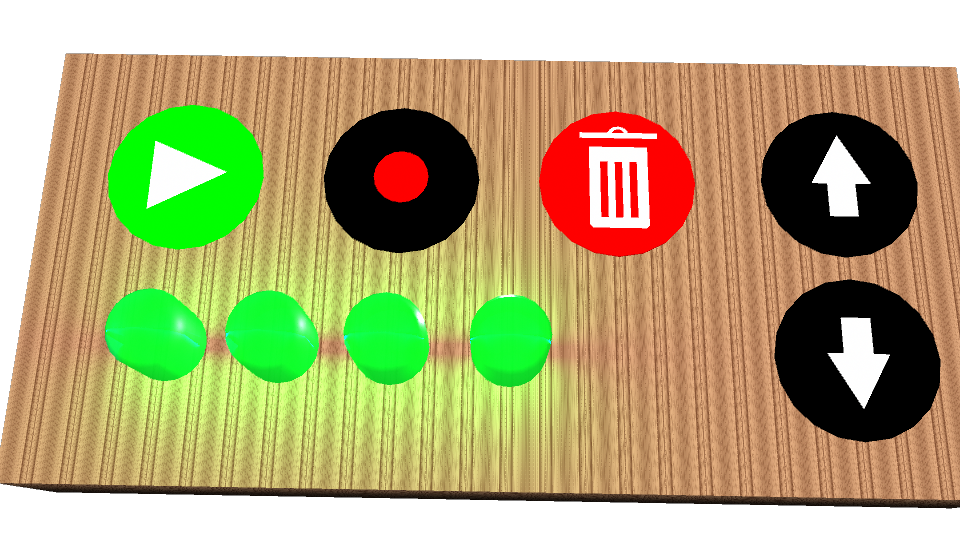
\includegraphics[width=0.7\linewidth]{figure/Design/buttonDesign}
	\label{fig:buttonDesign}
	\caption{The final design on how the buttons should look like and implemented on the prototype.}
	
\end{figure}


\subsection{Makings of the mat}

\begin{figure}[H]
	\centering
	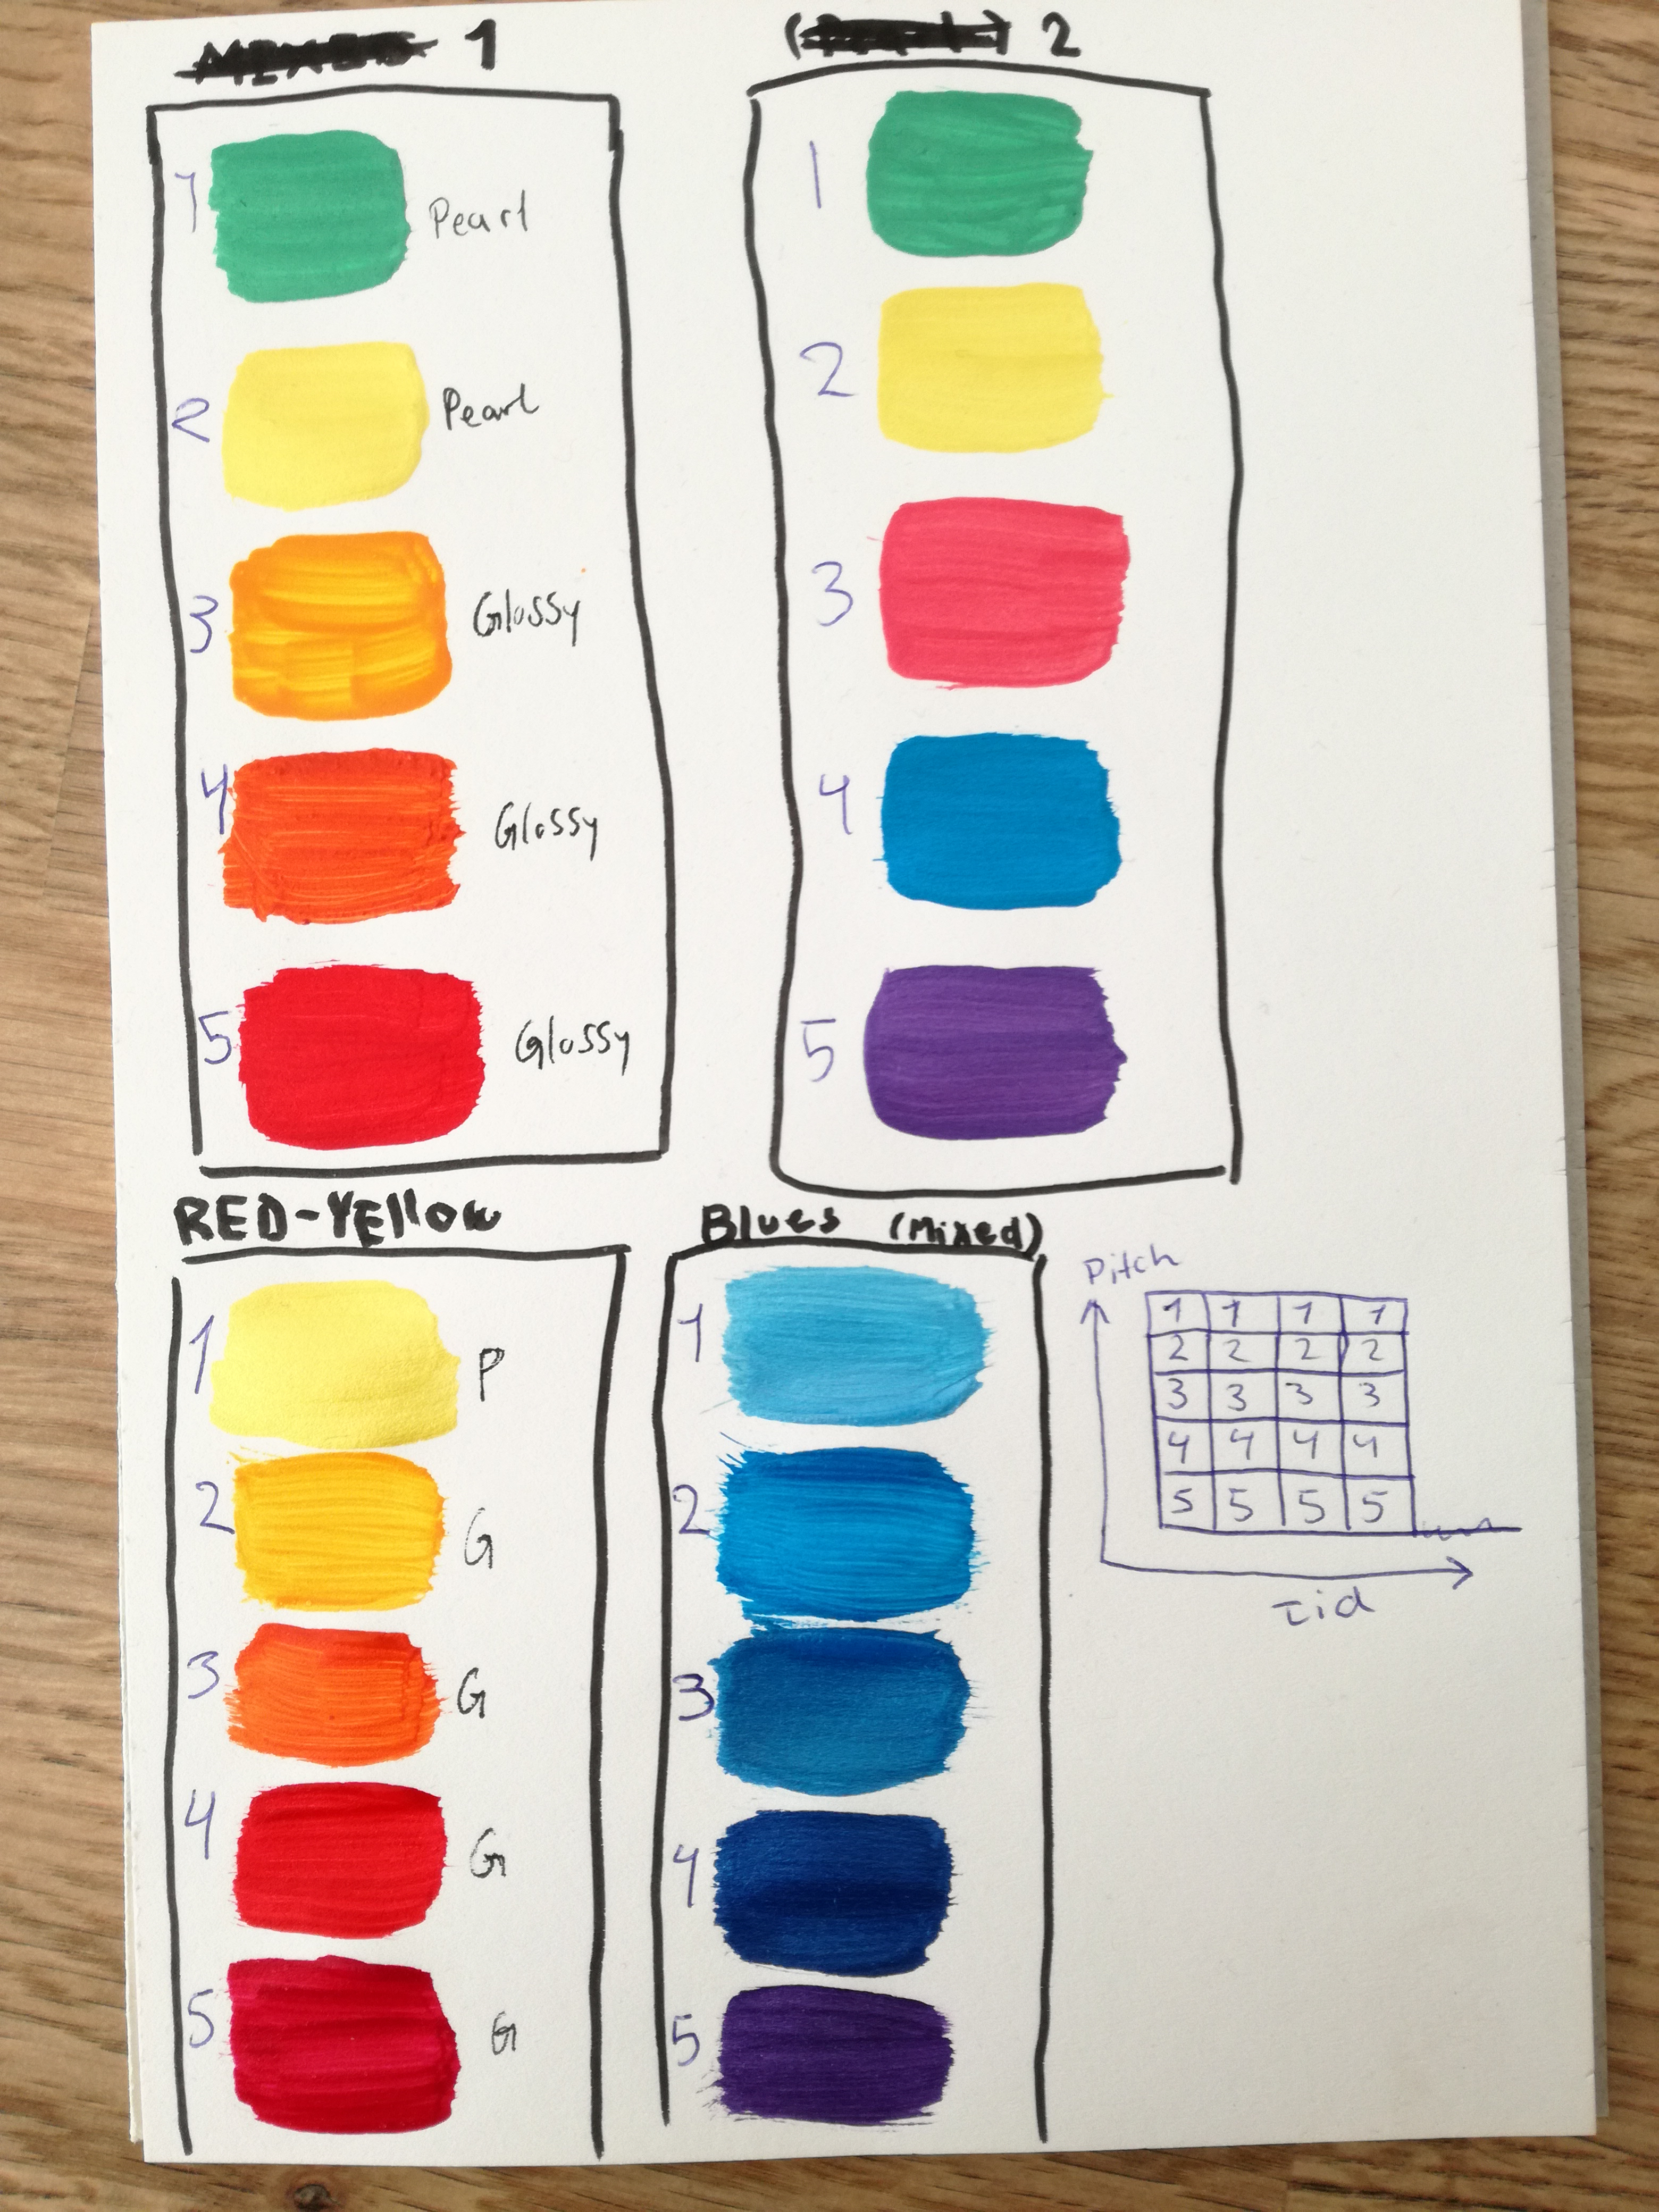
\includegraphics[width=0.5\linewidth]{figure/Design/colors}
	\label{fig:colors}
	\caption{The different color combinations for the mat}
	
\end{figure}

\section{The calculations}

\section{The result}













